% !TEX root = ../main.tex
\chapter{Architettura e responsabilità dei componenti}
\label{cap:architettura}

\section{Organizzazione a livelli e dipendenze}

\begin{figure}[!htbp]
    \centering
    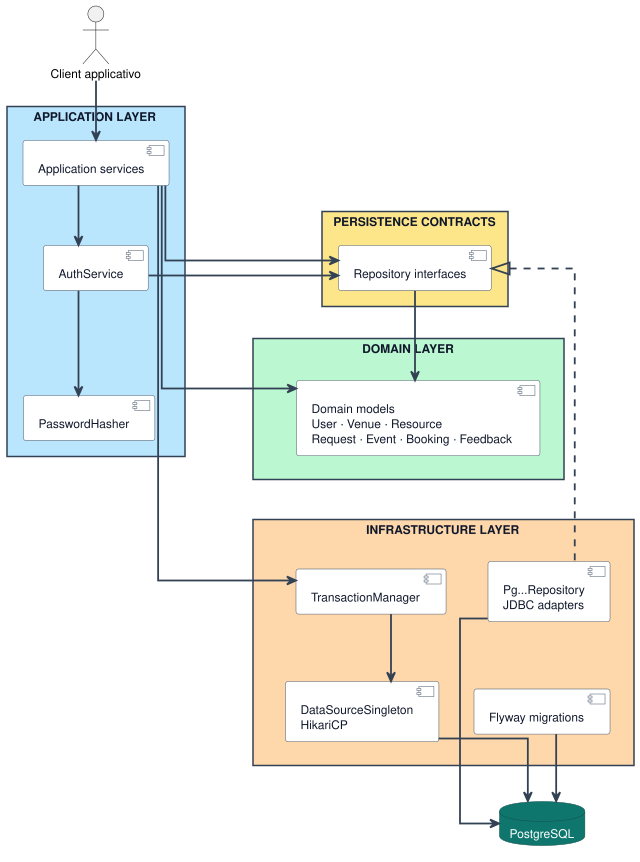
\includegraphics[width=\textwidth]{../docs/diagrams/architecture/layered-architecture.svg}
    \caption{Diagramma introduttivo dell'architettura a livelli.}
    \label{fig:layered-architecture}
\end{figure}

L'applicazione è organizzata su livelli che separano i modelli del dominio, i servizi applicativi e le implementazioni JDBC per la persistenza. I diagrammi offrono tre viste complementari: una vista logica per livelli, una sintesi delle dipendenze tra package Java e una vista di dettaglio dei componenti e dell'accesso al database. Le frecce indicano l'uso o la dipendenza tra componenti, non la sequenza temporale delle chiamate.

Il package \texttt{domain.model} contiene le classi e gli enum relativi agli utenti, alle venue, alle risorse, agli eventi, alle richieste, agli ospiti, alle prenotazioni e al feedback. I service utilizzano questi oggetti per rappresentare e trasferire i dati coinvolti nelle operazioni dell'app; il dominio è quindi indipendente rispetto all'implementazione dei service, dei repository e da PostgreSQL.

\begin{figure}[!htbp]
    \centering
    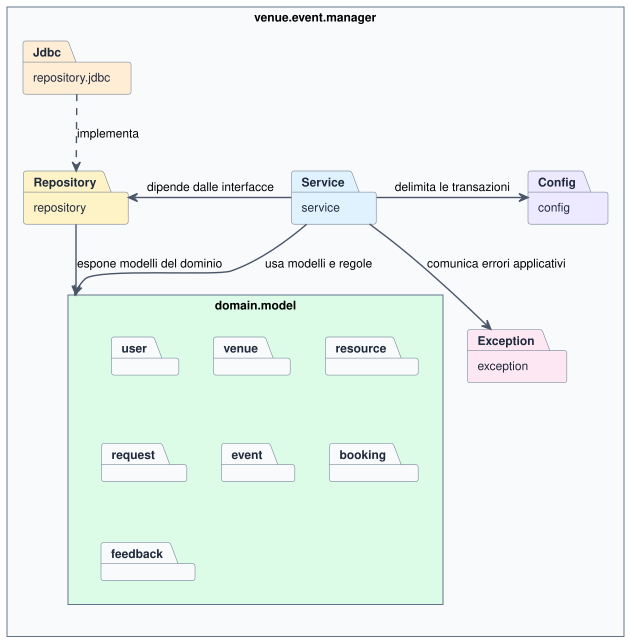
\includegraphics[width=\textwidth]{../docs/diagrams/architecture/package-dependencies.svg}
    \caption{Schema sintetico dei package Java e delle loro dipendenze.}
    \label{fig:package-dependencies}
\end{figure}

I service (contenuti nel package \texttt{service}) costituiscono il livello che si occupa di gestire i casi d'uso applicativi. I vari componenti dei service svolgono i controlli di validità, le verifiche di autorizzazione, le chiamate ai repository e la gestione delle transazioni necessarie. Le eccezioni applicative servono a rappresentare i problemi che si possono presentare durante l'esecuzione dell'app, come gli errori di validazione, i conflitti di stato, i divieti di accesso e l'assenza di dati.

La persistenza è effettuata attraverso l'uso delle interfacce nel package \texttt{repository}. I service dipendono da queste interfacce, evitando di contenere direttamente le query SQL. Le classi concrete del package \texttt{repository.jdbc} realizzano le interfacce e traducono le operazioni richieste in istruzioni JDBC.

Le interfacce dei repository lavorano esclusivamente con le entità del dominio e ricevono una \texttt{Connection} (da parte dei service) per eseguire le operazioni. Le implementazioni JDBC usano la connessione per interrogare o aggiornare PostgreSQL e, in base al caso, trasformano le righe restituite dal database in oggetti del dominio. Questo confine evita che i service dipendano direttamente dalle query, pur mantenendo JDBC incapsulato all'interno dei repository stessi.

Il coordinamento delle transazioni è gestito dal \texttt{TransactionManager}. I service definiscono il lavoro da eseguire tramite \texttt{inTransaction} (per le operazioni di scrittura) oppure \texttt{inReadOnly} (per le operazioni di lettura). Il \texttt{TransactionManager} acquisisce una connessione dal \texttt{DataSource}, gestisce commit e rollback e ripristina lo stato della connessione prima di restituirla al pool. In questo modo, più chiamate ai repository possono condividere la stessa connessione e, di conseguenza, appartenere alla medesima transazione.

Il \texttt{TransactionManager} è configurato per ottenere il \texttt{DataSource} da \texttt{DataSourceSingleton}, il quale carica i parametri tramite \texttt{DbConfig} e configura HikariCP per la gestione delle connessioni verso PostgreSQL. Le migrazioni di Flyway aggiornano lo schema in maniera separata dalle operazioni dell'app: esse, infatti, non vengono eseguite a ogni chiamata ai service.

\begin{figure}[!htbp]
    \centering
    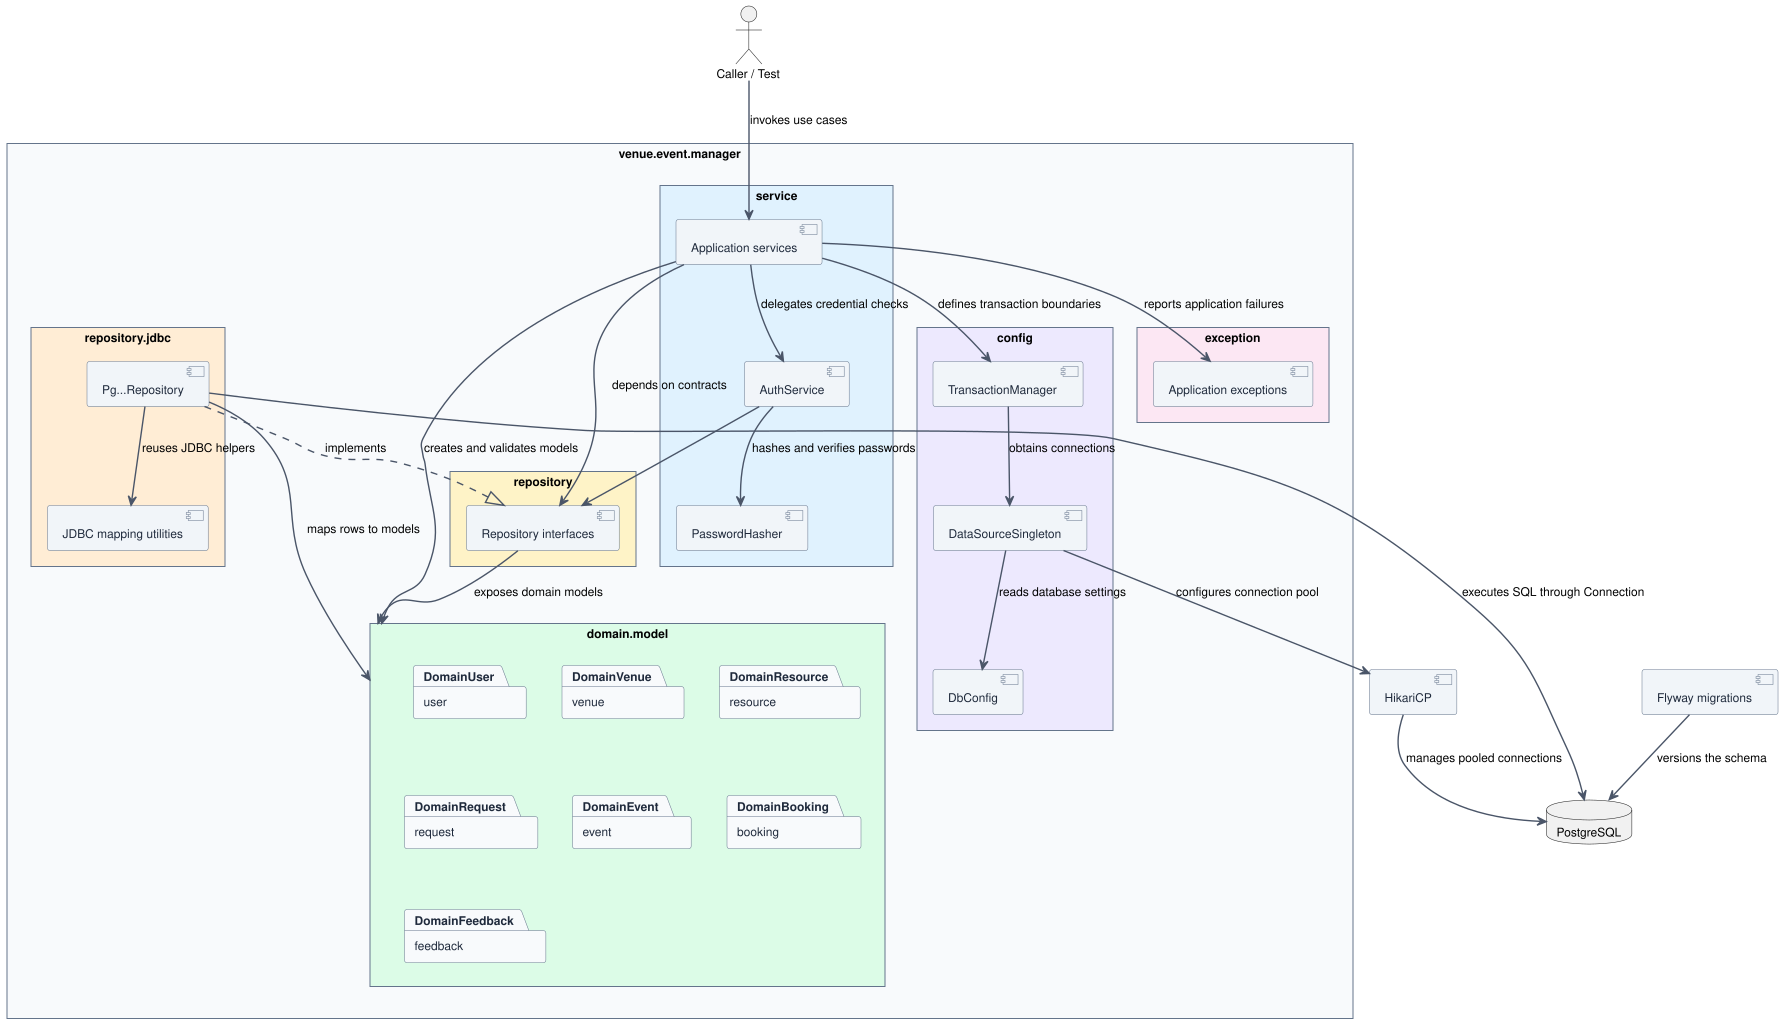
\includegraphics[width=\textwidth]{../docs/diagrams/architecture/package-architecture.svg}
    \caption{Schema dettagliato dei componenti e dell'accesso al database.}
    \label{fig:package-architecture}
\end{figure}

La configurazione del database è basata sulle variabili d'ambiente e sulle proprietà dell'app, in cui le prime hanno la precedenza sulle seconde. L'evoluzione dello schema è invece gestita da Flyway tramite script SQL versionati.

\texttt{AuthService} si occupa di gestire le credenziali tramite \texttt{UserRepository}, \texttt{TransactionManager} e \texttt{PasswordHasher}. Il modello \texttt{User} gestisce l'autenticazione tramite credenziali salvate separatamente. La verifica delle credenziali non crea una sessione né restituisce un token applicativo.

\section{Pattern e idiomi adottati}

La struttura dell'applicazione può essere descritta come un'architettura a livelli con Service Layer, Repository e dependency injection. Il Service Layer si occupa di gestire le operazioni applicative in maniera centralizzata; i repository separano le regole di accesso ai dati dalle implementazioni PostgreSQL. Questi elementi descrivono l'organizzazione e le responsabilità dei componenti, mentre la dependency injection tramite costruttore consente di sostituire le implementazioni, ad esempio nei test.

All'interno del dominio dei modelli è implementata l'immutabilità: i campi sono definiti come \texttt{final} e i metodi \texttt{with...} restituiscono una nuova istanza dell'oggetto con il valore modificato, senza alterare l'oggetto originale. Anche \texttt{Address} è un record immutabile. Gli aggiornamenti diventano così espliciti e le istanze già condivise non vengono mutate ''di nascosto''.

I metodi \texttt{inTransaction} (per modifiche/azioni sui dati) e \texttt{inReadOnly} (per letture sui dati) del \texttt{TransactionManager} applicano il paradigma ''Execute Around Method'': ricevono una funzione che descrive il lavoro sulla connessione e lo racchiudono nella gestione di apertura, commit o rollback e ripristino dello stato della connessione. Questo rende uniforme la gestione delle transazioni e riduce la duplicazione di codice infrastrutturale nei service.

Utilizziamo anche i pattern Singleton e Row Mapper. \texttt{DataSourceSingleton} e il \texttt{TransactionManager} condividono una singola istanza a livello applicativo, inizializzata solo alla prima invocazione (Lazy Initialization); \texttt{RowMapper<T>} associa una riga JDBC a una funzione (mapping del risultato di una query), utilizzabile anche tramite funzioni lambda, riducendo così la duplicazione nelle istanze condivise e nella conversione dei risultati JDBC.

Le macchine a stati delle entità non seguono il GoF State pattern: gli stati sono rappresentati tramite i valori enum delle singole entità e le transizioni ammesse sono verificate tramite i service. In maniera analoga, i modelli non sono costruiti con un builder dedicato, ma tramite costruttori e metodi \texttt{with...}. \texttt{TransactionManager} gestisce il confine delle transazioni, ma non mantiene un registro degli oggetti modificati e non costituisce una Unit of Work completa. Per questi motivi, la descrizione dell'architettura non viene estesa a pattern non implementati.

\section{Scelte e compromessi progettuali}

Il dominio del modello implementa l'immutabilità, che favorisce aggiornamenti espliciti e riduce i problemi che si possono verificare, al costo di creare una nuova istanza (che sostituisce quella vecchia) quando si modificano i dati. Questo approccio nel flusso esecutivo si traduce in: il service costruisce una copia e il repository si occupa di aggiornare la persistenza. La validazione e le transizioni sono responsabilità dei service, che non vengono quindi richieste ai modelli.

La dependency injection è gestita tramite i costruttori, il che rende esplicita la necessità dei service e consente di fornire dipendenze alternative nei test. L'istanza condivisa di \texttt{TransactionManager} viene usata in maniera predefinita, ma costruttori che accettano un manager esplicito permettono invece di verificare il confine delle transazioni. Questa soluzione permette di mantenere semplice la struttura dell'applicazione, senza introdurre un framework di dependency injection.

L'utilizzo delle interfacce repository limita l'associazione fra i service e le query specifiche di PostgreSQL e rende possibile sostituire gli adapter nei test. Il confine non è tuttavia completamente indipendente dall'infrastruttura: i metodi dei repository ricevono \texttt{java.sql.Connection}, necessaria per condividere la connessione e la transazione correnti. Questa scelta esplicita il controllo delle transazioni e semplifica l'esecuzione di più operazioni atomiche, ma espone ai contratti un tipo JDBC.

L'architettura è quindi organizzata a livelli, con contratti per i repository e adapter JDBC, senza essere un'architettura esagonale formale. Non sono presenti port e adapter applicativi espliciti per una UI o un'API: i service sono attualmente il punto di accesso alle funzionalità del nucleo applicativo.